\documentclass[10pt]{jarticle}
\usepackage{ascmac}
\usepackage[dvipdfmx]{graphicx}
\usepackage{enumerate}
\usepackage{amsmath,amssymb}
\usepackage{url}
\usepackage{enumitem}
\usepackage{listings}
\usepackage[hang,small,bf]{caption}
\usepackage[subrefformat=parens]{subcaption}
\renewcommand{\lstlistingname}{source}
\lstset{language=sh,%
        basicstyle=\footnotesize,%
	commentstyle=\textit,%
	classoffset=1,%
	keywordstyle=\bfseries,%
	frame=shadowbox,framesep=4pt,%
	showstringspaces=false%,
	numbers=left,stepnumber=1,numberstyle=\footnotesize,%
	numbersep=1zw,%
	lineskip=-0.5ex,%
	xleftmargin=2zw%
	}%

\newdimen\paperwidth \newdimen\paperheight
\def\A4size{\paperwidth=210mm \paperheight=297mm}
\def\centered{%
  \oddsidemargin=\paperwidth
  \advance\oddsidemargin-\textwidth
  \oddsidemargin=0.5\oddsidemargin
  \advance\oddsidemargin-1in
  \evensidemargin-\oddsidemargin}
%
\textwidth 160mm
\textheight 230mm
\topmargin 0mm
\headheight 0mm
\footskip 0mm
\A4size\centered

\title{\framebox{\hspace{4zw}データ科学 レポート3%
                 \hspace{4zw}}}
\author{神野 友哉 \\
        2022311042  \\
        愛知県立大学 情報科学部 情報科学科 \\}
\date{2023年12月17日}


\begin{document}
\maketitle
\tableofcontents
\clearpage

\section{はじめに}
%
この実験では、\ MapReduce\ 法によって、メモリに収まらない程大きいデータが扱えるようになることを学ぶ。
更に、実際にビッグデータを処理することで、活用方法も理解する。

%
\section{課題 1}
%

作業\ 1\ ～\ 2\ を行う。処理時間計測の際、必ず実行二回目を記録する。
\begin{itemize}[left=30pt]
\item[[作業1]] \ \verb|program_m1.m|、\ map関数、\ reduce関数、\ mapimage.m\ を作成して\ MapReduce\ の逐次処理を行い、処理時間を計測する
\item[[作業2]] \ \verb|program_m2.m|\ を作成して\ MapReduce \ の並列処理を、\ 2、\ 4、\ 6、\ 8、\ 12、\ 16\ 並列で
行い、処理時間を計測する。
\end{itemize}
作業\ 1\ の\verb|program_m1.m|はプログラム\ref{tikuji}、作業\ 2\ の\verb|program_m2.m|はプログラム\ref{heiretu}、\ map関数、\ reduce関数、\ mapimage.m\
は、それぞれプログラム\ref{map1}、\ref{reduce1}、\ref{mapimage}である。
\lstinputlisting[caption=programm\_1.m (逐次処理),label=tikuji]{programm1distribute.m}
\lstinputlisting[caption=programm\_2.m (並列処理),label=heiretu]{programm2.m}
\lstinputlisting[caption=map関数,label=map1]{statmapper.m}
\lstinputlisting[caption=reduce関数,label=reduce1]{statreducer.m}
\lstinputlisting[caption=mapimage.m,label=mapimage]{mapimage.m}
%

\subsection{課題 1-1}
	作業\ 1,\ 2\ の結果を利用して、コア数毎\ ( $N\ge 2$)\ に、計算時間\ ($t_{n}$)、速度向上度\ ($S_{n}$)、
	Karp-Flatt\ metric\ \ ($K_{f}$)\ を計算し、結果を折れ線グラフ\ (横軸は並列数)\ でプロットせよ
\subsubsection{目的}
%
\ MapReduce\ 法の並列処理の効果を確かめる。
%

\subsubsection{考察}
%
プログラム\ref{tikuji}を実行し、その処理時間が逐次処理時間となる。その後、\ Parpool($N$)\ で設定したワーカー数で
プログラム\ref{tikuji}と同様の処理を並列で行うプログラム\ref{heiretu}を実行し、
並列処理時間のデータを得る。逐次処理時間と各並列処理時間を比較する。
結果は表\ref{table:11}になった。
\begin{table}[htbp]
	\centering
	\caption{処理時間の観測結果}
	\label{table:11}
	\begin{tabular}{|c|c|c|c|c|c|c|c|c|}
		\hline
		$N$ & 1 (逐次処理) & 2 & 3 & 4 & 5 & 6 & 7 & 8 \\
		\hline
		$t_{n}$(s) & 48.7170 ($t_{s}$) & 22.5342 & 17.2881 & 15.9825 & 11.5062 & 10.0785 & 9.0965 & 8.3843 \\
		\hline
    $N$ & 9 & 10 & 11 & 12 & 13 & 14 & 15 & 16 \\
		\hline
		$t_{n}$(s) & 7.6002 & 7.1209 & 7.0618 & 6.9421 & 6.2595 & 6.1114 & 6.0952 & 6.2074 \\
		\hline
	\end{tabular}
\end{table}
表\ref{table:11}を見ればすぐに判ることだが、並列処理のコア数$ N $が増加するにつれて、処理時間は($ N=16 $を除いて)単調減少である。
そのため、\ MapReduce\ 法の並列処理によって高速化されていると考えてよい。本題に入るが、
得られた処理時間のデータから、速度向上度\ ($S_{n}= \frac{t_{s}}{t_{n}}, t_{s}は逐次処理時間 t_{1}$)を計算したものが表\ref{table:12}である。
\begin{table}[htbp]
	\centering
	\caption{速度向上度\ ($S_{n}$)\ の計算結果}
	\label{table:12}
	\begin{tabular}{|c|c|c|c|c|c|c|c|c|}
		\hline
		$N$ & 1 (逐次処理) & 2 & 3 & 4 & 5 & 6 & 7 & 8 \\
		\hline
		$S_{n}$ & 1 & 0.4626 & 0.3549 & 0.3281 & 0.2362 & 0.2069 & 0.2069 & 0.1867 \\
		\hline
    $N$ & 9 & 10 & 11 & 12 & 13 & 14 & 15 & 16 \\
		\hline
		$S_{n}$ & 0.1560 & 0.1462 & 0.1450 & 0.1450 & 0.1285 & 0.1254 & 0.1251 & 0.1274 \\
		\hline
	\end{tabular}
\end{table}
更に、プログラム\ref{keisan}を実行することにより、速度向上度\ ($S_{n}$)\ から\ Karp-Flatt\ metric\ \ ($K_{f}$)\ 
を計算し、$ N $に対してプロットしたものが、図\ref{fig:wk3-1}である。
\begin{figure}[htbp]
	\begin{center}
		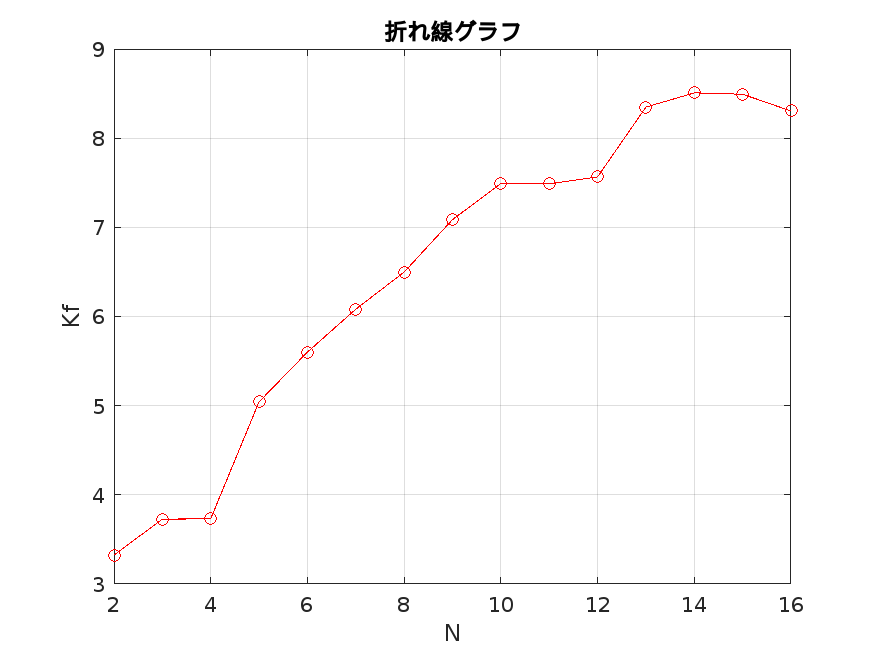
\includegraphics[width=70mm]{wk2-1.png}
	\end{center}
	\caption{$N$ と $K_{f}$の関係}
	\label{fig:wk3-1}
\end{figure}
図\ref{fig:wk3-1}から、$ N = 14 $までは$ K_{f} $は増加傾向にあると考えられるが、$ N = 14 $から減少しているため、
$ N = 14 $周辺が取りえる最大となるのではないか。

\newpage
\lstinputlisting[caption=計算とプロット,label=keisan]{cal21.m}
%

\subsubsection{結論}
%
この実験で用いたプログラムの処理では、\ MapReduce\ 法による効率化が確認された。しかし、並列処理のコア数$ N $
を無尽蔵に増やす必要はないと結論づけてよいだろう。
%

\subsection{課題 1-2}
%
\ MapReduce\ のアルゴリズムの利点・欠点について調査せよ
%

\subsubsection{目的}
%
\ MapReduce\ 法の使うべき場合とそうでない場合を見極めるには、そのアルゴリズムの利点・欠点を知る必要があるため。
%

\subsubsection{考察}
%
\ MapReduce\ 法の利点として、巨大なデータを分割してメモリに読み込み、計算を実施するため、
メモリの上限を上回るような巨大なデータを扱えるようになる。欠点として、データがメモリに収まるような場合は、効率化が見込めない。
また、巨大なデータを構成する微細なデータ同士が複雑に関係する場合も非効率な場合もある。
%

\subsubsection{結論}
%
\ MapReduce\ 法は、メモリよりも大きいデータ(ビッグデータ)で活用するべきである。
%

\section{課題 2}
%
\ 16\ 並列による\ MapReduce\ 処理を利用し、
ニューヨークのイエローキャブ利用のビッグデータから、
料金や走行距離、昇降地点等の情報を可視化する。
それによって得られた図から、データの分析を行う。

%

\subsection{課題 2-1}
%
プログラム\ref{heiretu}をコピーして、読み込み対象のデータを\ 2017\ 年\ 1\ 月から\ 12\ 月までとなるよう修正した
プログラム\ref{ryokin1}を作成せよ。その後、処理結果\verb|(fare_ave)|を\ プログラム\ref{mapimage}\ により可視化して得られる図を示せ。
また、その図と地域の土地利用に関する特徴を調べて見比べ、今回の結果が得られた理由を考察せよ。ただし、土地利用に関する特徴は、
\ GoogleMap\ 等のウェブ上で閲覧可能な地図アプリケーション等を利用してよい。
\lstinputlisting[caption=料金(1年分16並列),label=ryokin1]{programm3.m}
%

\subsubsection{目的}
%
ニューヨークのイエローキャブの利用料金と都市の土地の利用との関連を調べる。
%

\subsubsection{考察}
%
図\ref{fig:wk3-2}は、プログラム\ref{ryokin1}を実行したのち、
コマンドラインで\ \verb|mapimage(fare_ave,id)|\ とタイプして実行した結果である。
また、図\ref{fig:newyork}は、ニューヨークの最も有力な交通として一日360万人に利用されるニューヨーク地下鉄である。これは、
ニューヨークの中心部マンハッタンとブルックリンに多くの路線が通っている。
\begin{figure}[htbp]
  \begin{minipage}{0.3\textwidth}
    \begin{center}
      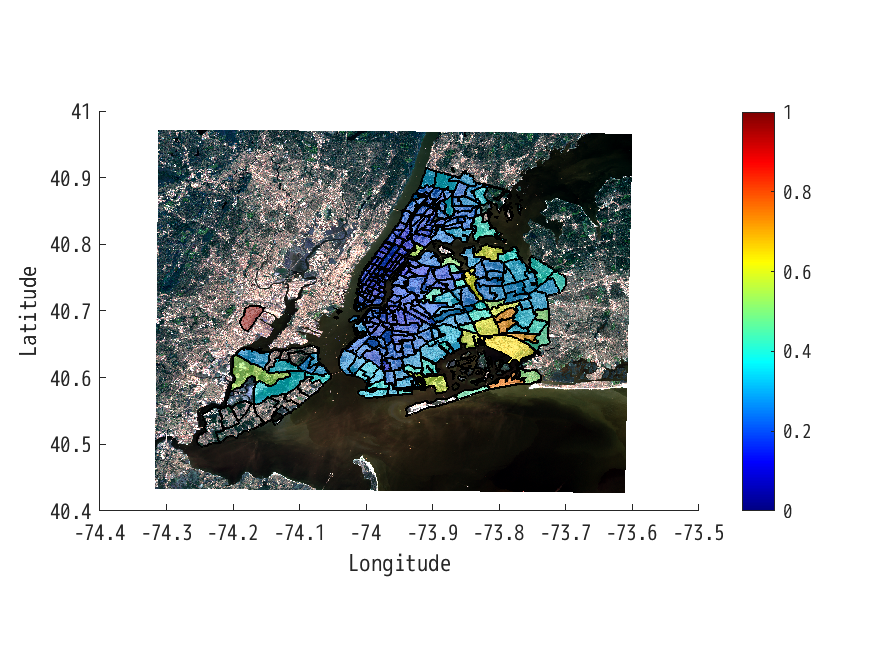
\includegraphics[width=33mm]{kadai2-1.png}
    \end{center}
    \subcaption{ニューヨークの土地とイエローキャブの利用料金(1年)}
    \label{fig:wk3-2}
  \end{minipage}
  \begin{minipage}{0.3\textwidth}
    \begin{center}
      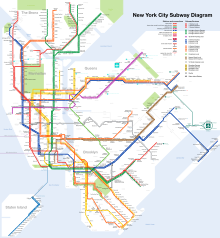
\includegraphics[width=33mm]{NYC_subway-4D.svg.png}
    \end{center}
    \subcaption{ニューヨークの地下鉄路線図}
    \label{fig:newyork}
  \end{minipage}
  \begin{minipage}{0.3\textwidth}
    \begin{center}
      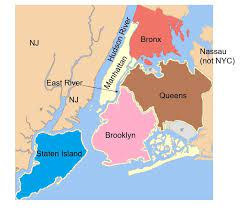
\includegraphics[width=33mm]{kub.jpg}
    \end{center}
    \subcaption{ニューヨークの区}
    \label{fig:CGcylinder}
  \end{minipage}
  \caption{ニューヨークのイエローキャブ利用についての資料}
  \label{fig:siryou}
\end{figure}

図\ref{fig:siryou}から見て取れるのは、地下鉄の路線の密集度合いがイエローキャブの利用料金に負の相関関係があるということである。
その原因を考察する。ニューヨーク中心部における地下鉄の利用料金が一律2.9ドルと、イエローキャブのそれに対し価格優位であることや、
公共交通機関の定時制(日本のそれと比べていい加減な面も否定できないが)が挙げられるのではないか。
国土交通省の昭和62年度運輸白書によると、都市部では通勤・通学の際に公共交通機関が多く利用されるという\cite{kokudo}。
日本の国家機関のデータではあるが、今回の実験の結果の理由として援用できるのではないか。
%

\subsubsection{結論}
%
ニューヨーク中心部も日本の都会のそれと同様に、公共交通機関が利用される傾向にあると考えられる。
%

\subsection{課題 2-2}
%
\ 2017\ 年\ 1\ 月から\ 12\ 月までのデータを対象に、\ \verb|trip_distance|(走行距離)のデータを用いて単位距離当たりの料金
(料金の総和を距離の総和で除したもの)を\ PULocationID\ ごとに求め、プログラム\ref{mapimage}により可視化せよ。
また、可視化した結果と地域の土地利用に関する特徴を調べ、今回の結果が得られた理由を考察せよ。ただし、支払料金が\ 0\ ドル以下または\ 300\ 
ドルより大きい、または、走行距離が\ 0.5\ km\ 以下または\ 100\ km\ より大きいものは除外すること。
%

\subsubsection{目的}
%
料金や走行距離のはずれ値を除外したデータを用いることで、より実態に沿った考察をしやすくするため。
%

\subsubsection{考察}
%
課題\ 2-2\ のために走行距離のデータを処理できるよう、プログラム\ref{ryokin1}、\ref{map1}、\ref{reduce1}から
それぞれプログラム\ref{ryokin2}、\ref{map2}、\ref{reduce2}を作成した。
\lstinputlisting[caption=単位距離当たりの料金(1年分16並列),label=ryokin2]{programm4.m}
\lstinputlisting[caption=はずれ値を除いたmap関数,label=map2]{statmapper2.m}
\lstinputlisting[caption=はずれ値を除いたreduce関数,label=reduce2]{statreducer2.m}

図\ref{fig:wk3-3}は、プログラム\ref{ryokin2}を実行したのち、
コマンドラインで\ \verb|mapimage(fare_ave,id)|\ とタイプして実行した結果である。
\begin{figure}[htbp]
	\begin{center}
		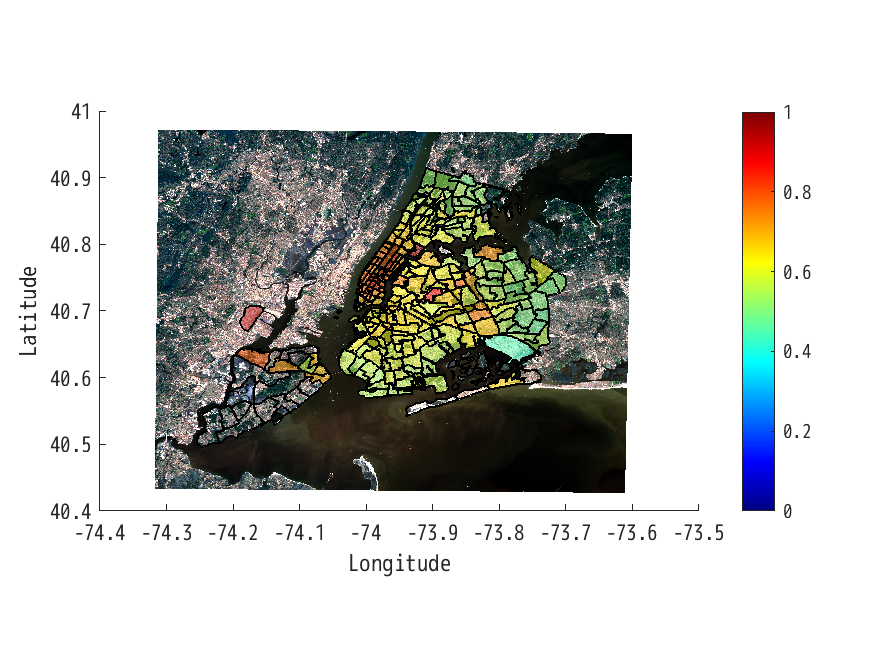
\includegraphics[width=75mm]{kadai2-2.png}
	\end{center}
	\caption{ニューヨークの土地とイエローキャブの単位距離当たりの料金(1年)}
	\label{fig:wk3-3}
\end{figure}

図\ref{fig:wk3-3}はまるで図\ref{fig:wk3-2}の色相を逆にした様であった。
この原因を考察する。ニューヨークの中心部マンハッタンの単位距離当たりの料金が高かった原因は、
マンハッタンが経済の中心であるため、利用する人が多く存在することが考えられる。
また、憶測でしかないが、ニューヨーク州のイエローキャブが初乗り\ 2.5\ ドルで\ 1.5\ マイル(約320m)おきに
\ 0.5\ ドルずつ増加するため、少しでも安く済ませようと
メーターが増加しないギリギリで降り、目的地までの残りを徒歩で歩く人がそこそこの割合でいるのではないか。
%

\subsubsection{結論}
%
ニューヨークの中心部マンハッタンでの客単価が高いことが判明した。
%

\begin{thebibliography}{5}
  \bibitem{mathlab1}
    MathWorks: "MapReduce 入門", MathWorks. 2023, \\
    \url{https://jp.mathworks.com/help/matlab/import_export/getting-started-with-mapreduce.html}, (参照 2023-12-17).
	\bibitem{nikkei}
		世界お値段調査隊: "NY地下鉄初乗り420円 幻じゃない!?改札の「ゴースト」", 日経新聞. 2023, \\
		\url{https://www.nikkei.com/article/DGXZQOGN2602Y0W3A820C2000000/#:~:text=1%E6%97%A5%E5%BD%93%E3%81%9F%E3%82%8A%E3%81%AE%E4%B9%97%E5%AE%A2%E6%95%B0,%E3%81%99%E3%82%8B%E8%A6%B3%E5%85%89%E5%9C%B0%E3%81%A7%E3%82%82%E3%81%82%E3%82%8A%E3%81%BE%E3%81%99%E3%80%82}, (参照 2023-12-17).
	\bibitem{kokudo}
    国土交通省: "1 都市交通の整備", 国土交通省. 1987, \\
    \url{https://www.mlit.go.jp/hakusyo/transport/shouwa62/ind000502/001.html}, (参照 2023-12-17).
\end{thebibliography}
\end{document}
